\documentclass[tikz]{standalone}
\usepackage{amsmath}

\usetikzlibrary{tqft,calc}

\begin{document}

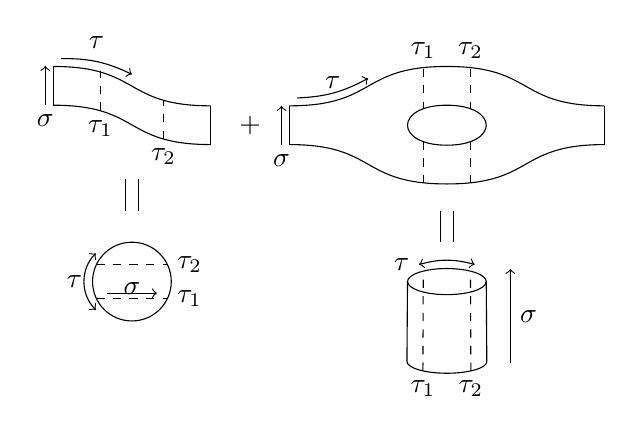
\begin{tikzpicture}[
    every tqft/.append style={
        transform shape, rotate=90, tqft/circle x radius=7pt,
        tqft/circle y radius=0pt, tqft/boundary separation=1cm
      }
  ]

  % cobordism at upper left
  \pic[
    tqft/cylinder to prior,
    name=a,
    every outgoing lower boundary component/.style={draw},
    every incoming boundary component/.style={draw},
    cobordism edge/.style={draw},
  ];

  % annotation of cobordism at upper left
  \coordinate (temp1) at ($(a-incoming boundary.west)!0.3!(a-outgoing boundary.west) +(0,0.08)$);
  \coordinate (temp2) at ($(a-incoming boundary.west)!0.7!(a-outgoing boundary.west) +(0,-0.08)$);
  \draw[dashed]
  (temp1) node[below] {$\tau_1$} -- +(0,0.5)
  (temp2) node[below] {$\tau_2$} -- +(0,0.5);
  \draw[->] ($(a-incoming boundary.west) - (0.1,0)$) node[below] {$\sigma$} -- ++(0,0.5);
  \draw (a-outgoing boundary) ++(0.5,0) node {$+$};
  \draw[->] ($(a-incoming boundary.east)+(0.1,0.1)$) to[bend left=13] +(0.9,-0.2);
  \node[above] at ($(a-incoming boundary.east)+(0.55,0.1)$) {$\tau$};

  % cobordism at upper right consisting of two 'pants'
  \pic[
    tqft/pair of pants,
    name=b,
    every incoming upper boundary component/.style={draw},
    every incoming boundary component/.style={draw},
    cobordism edge/.style={draw},
    at={($(a-outgoing boundary)+(1,0)$)},
  ];

  \pic[
    tqft/reverse pair of pants,
    name=c,
    every outgoing lower boundary component/.style={draw},
    % every incoming boundary component/.style={draw},
    cobordism edge/.style={draw},
    at=(b-outgoing boundary 1),
  ];

  % annotation of cobordism at upper right
  \draw[->] ($(b-incoming boundary.west) - (0.1,0)$) node[below] {$\sigma$} -- ($(b-incoming boundary.east) - (0.1,0)$);
  \coordinate (temp1) at ($(b-between outgoing 1 and 2)!0.2!(c-between incoming 1 and 2) +(0,0.72)$);
  \coordinate (temp2) at ($(b-between outgoing 1 and 2)!0.8!(c-between incoming 1 and 2) +(0,0.72)$);
  \draw[dashed]
  (temp1) node[above] {$\tau_1$} -- +(0,-0.51) ++(0,-0.93) -- ++(0,-0.53)
  (temp2) node[above] {$\tau_2$} -- +(0,-0.51) ++(0,-0.93) -- ++(0,-0.53);
  \draw[->] ($(b-incoming boundary.east)+(0.1,0.1)$) to[bend right=13] +(0.9,0.25);
  \node[above] at ($(b-incoming boundary.east)+(0.55,0.1)$) {$\tau$};

  % drawing cylinder
  \path let \p1=(b-between outgoing 1 and 2), \p2=(c-between incoming 1 and 2) in
  node[name=cyl1, minimum width={\x2-\x1}] at ($(b-outgoing boundary 1)-(0,2.5)$) {}
  node[name=rec,shape=rectangle, minimum height=1cm, minimum width={\x2-\x1}, anchor=south]
  at (cyl1) {}
  node[name=cyl2,shape=ellipse, minimum height=.3cm, minimum width={\x2-\x1}, draw, outer sep=0]
  at (rec.north) {}
  ;
  \draw (cyl1.west) -- (cyl2.west) % left side
        (cyl1.east) -- (cyl2.east) % right side
        (cyl1.west) arc(-180:0:0.508cm and 0.15cm); % bottom ellipse

  % annotating cylinder
  \draw[<->] ($(cyl2.north east)+(0,0.1)$) to[bend right=15] ($(cyl2.north west)+(0,0.1)$);
  \node[left] at ($(cyl2.north west)+(0,0.1)$) {$\tau$};
  \draw[->] (cyl1.south east) ++ (0.3,0.1) -- ++(0,1.2);
  \draw (cyl1.south east) ++ (0.3,0.7) node [right] {$\sigma$};
  \draw[dashed] ($(cyl1.west)!0.2!(cyl1.east) +(0,-0.12)$) node[below] {$\tau_1$} --($(cyl2.west)!0.2!(cyl2.east) +(0,0.12)$)
  ($(cyl1.west)!0.8!(cyl1.east) +(0,-0.12)$) node[below] {$\tau_2$} --($(cyl2.west)!0.8!(cyl2.east) +(0,0.12)$);
  \draw (cyl2) ++(85:0.9) -- +(0,-0.4) (cyl2) ++(95:0.9) -- +(0,-0.4);
  % drawing and annotating circle
  \node[draw, shape=circle, minimum width=1cm]
  at (cyl2.west -| a-between first incoming and first outgoing) (circ) {};
  \draw[dashed] (circ) +(155:0.5) -- +(25:0.5) node[right] {$\tau_2$}
  +(205:0.5) -- +(335:0.5) node[right] {$\tau_1$};
  \draw[->] (circ) +(205:0.35) -- +(335:0.35);
  \node[below=-0.3em] at(circ) {$\sigma$};
  \draw (circ) ++(85:0.9) -- +(0,0.4) (circ) ++(95:0.9) -- +(0,0.4);
  \draw[<->] (circ.south west) +(-0.1,0) to[bend left=45] ($(circ.north west)+(-0.1,0)$);
  \node[left] at(circ.west) {$\tau$};
\end{tikzpicture}

\end{document}
